\documentclass{article}

% if you need to pass options to natbib, use, e.g.:
% \PassOptionsToPackage{numbers, compress}{natbib}
% before loading nips_2016
%
% to avoid loading the natbib package, add option nonatbib:
% \usepackage[nonatbib]{nips_2016}

\usepackage[final]{nips_2016}

% to compile a camera-ready version, add the [final] option, e.g.:
% \usepackage[final]{nips_2016}

\usepackage[utf8]{inputenc} % allow utf-8 input
\usepackage[T1]{fontenc}    % use 8-bit T1 fonts
\usepackage{hyperref}       % hyperlinks
\usepackage{url}            % simple URL typesetting
\usepackage{booktabs}       % professional-quality tables
\usepackage{amsfonts}       % blackboard math symbols
\usepackage{nicefrac}       % compact symbols for 1/2, etc.
\usepackage{microtype}      % microtypography
\usepackage{graphicx}
\usepackage{subfig}
\usepackage{placeins}


\title{RSGAN: Recurrent Stacked Generative Adversarial Network for Conditional Video Generation}

% The \author macro works with any number of authors. There are two
% commands used to separate the names and addresses of multiple
% authors: \And and \AND.
%
% Using \And between authors leaves it to LaTeX to determine where to
% break the lines. Using \AND forces a line break at that point. So,
% if LaTeX puts 3 of 4 authors names on the first line, and the last
% on the second line, try using \AND instead of \And before the third
% author name.

\author{
  Shujon Naha, Khandokar Md. Nayem,  Md. Lisul Islam
  \vspace*{0.5em}\\
  School of Informatics and Computing\\
  Indiana University\\
  Bloomington, IN \\
  \texttt{ \{snaha, knayem, islammdl\}@iu.edu} \\
}

%\author{
%  Shujon Naha \\
%  Department of Computer Science\\
%  Indiana University\\
%  Bloomington, IN \\
%  \texttt{snaha@iu.edu} \\
%  %% examples of more authors
%   \And
%   Khandokar Md. Nayem \\
%  Department of Computer Science\\   
%  Indiana University\\
%  Bloomington, IN \\
%   \texttt{knayem@iu.edu} \\
%   \AND
%   Md. Lisul Islam\\
%  Department of Computer Science\\   
%  Indiana University\\
%  Bloomington, IN \\
%   \texttt{islammdl@indiana.edu } \\
%}

\begin{document}
% \nipsfinalcopy is no longer used

\maketitle

\begin{abstract}
  Generating video frames based on a pre-condition is a challenging problem and requires understanding of per frame contents and visual dynamics and their relevacies to the pre-condition. In this paper, we propose a novel Recurrent Stacked Generative Adversarial Network (RSGAN) based model to generate video frames based on a given pre-condition. The pre-condition can be anything related to the generated video, like- action classes, sentence descriptor, fMRI signal, etc. In our knowledge, this is the first work to address the problem of conditional video generation using adversarial network.
\\\\
\textbf{Index Terms:} rsgan, recurrent netwok, stacked generative adversarial network, adversarial network, conditional video generation, video generation. 
\end{abstract}

%%%%%%%%%%%%%%%%%%%%%%%%%%%%%%%%%%%%
%
%				Section: Introduction
%
%%%%%%%%%%%%%%%%%%%%%%%%%%%%%%%%%%%%
\section{Introduction}
\label{introduction}
Generative adversarial networks have been shown incredible results to produce images from pre-conditions such as text, attributes etc \cite{stackGAN, attribute2image}. In these works, random noises incorporated with a semantic vector representation of the prec-condition is given as input to the generator network to produce images relevant to the pre-condition. The discriminator network then learns to distinguish between the images generated by the generator and the real image from the database. A min-max learning algorithm is used to train these both models where the generator tries to continously fool the discriminator by producing better images similar to the original one and the discriminator learns to make the job harder for the generative network by getting better at distinguishing real and fake images. Most of the times, the generative network is a convolutional neural network which produces image from a single vector by using several deconvolution steps. The discriminator network is also a convolutional neural network which takes the image from the generator network output and the corresponding original image from the database and tells the similarity between the generated image and the real image. 


Generative adversarial networks have been also used for predicting future frames from a video sequence and generate videos with scene dynamics \cite{deepMSE, genVSD}. In this works, multiple frames are combined together and 3D convolution is used in the domains of space and time to predict the next frames. These works have shown the capability of adversarial networks to capture the scene dynamics although for small temporal intervals.

\begin{figure}[h]
  \centering
  %%\fbox{\rule[-.5cm]{0cm}{4cm} \rule[-.5cm]{4cm}{0cm}}
  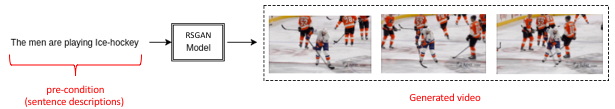
\includegraphics[scale=0.45]{problem1.png} 
  \caption{Generating video sequence based on a given pre-condition (sentence description).}
    \label{problem}
\end{figure}

In this paper, we address the problem of generating videos based on pre-conditions such as action classes, fMRI signals and sentence descriptions using adversarial network. Generating videos based on pre-conditions pose a unique set of challenges than the conditional image generation and unconditional video generation problem. In our case, each of the frames will be generated based on the previous frames and the given pre-condition such as in Figure \ref{problem}. The numbers of previous frames can vary from zero to a maximum number. Thus the usual approach of using 3D convolution will not be applicable in our case. Moreover, we need to make the pre-condition available to the system at each time frame so the whole generated video is consistent with the pre-condition.    


%%%%%%%%%%%%%%%%%%%%%%%%%%%%%%%%%%%%
%
%				Section: Background
%
%%%%%%%%%%%%%%%%%%%%%%%%%%%%%%%%%%%%
\section{Background}
\label{background}
In this section will review FCN, RNN and GAN which will be repeatedly referred to through the paper.

\subsection{Fully Convolutional Networks (FCN)}
\label{fully_convolutional_networks}
For classification task using convolutional neural networks, the few last fully connected layers
are responsible for the classification part. But with pixel-wise labelling, there is a need for dense predictions on all the pixels. In \cite{deepSeg2015} the idea of using a fully convolutional neural network that is trained for pixel-wise semantic segmentation is presented. It is shown that it surpasses the state of the art in semantic segmentation on PASCAL VOC, NUYDv2, and SIFT Flow datasets. The FCN method is briefly discussed in what follows.
\\\\
FCN architecture is based on VGG \cite{deepConv2014} architecture due to its success in classification tasks. However, due to the fully connected layers that these networks have, they can only accept fixed size input and produce a classification label. To overcome this problem, it is possible to convert a fully connected layer into a convolutional layer. Accordingly, this network can yield coarse maps pixel wise prediction instead of one classification output.
\\\\
In order to have dense prediction from this coarse map, it needs to be up-sampled to the original size of the input image. The up-sampling method can be a simple bi-linear interpolation. But in \cite{deepSeg2015} a new layer that applies upsampling within the network was presented. It makes it efficient to learn the up-sampling weights within the network using back-propagation. The filters of the deconvolution layer act as the basis to reconstruct the input image. Another idea for up-sampling is to stitch together output maps from shifted version of the input. But It was mentioned in \cite{deepSeg2015} that using up-sampling with deconvolution is more effective. In [18] the idea of having a full deconvolution network with both deconvolution layers and unpooling layers is presented.
\\\\
The FCN architecture has been tried in different applications. In \cite{densebox2015} it is used for object localization. In \cite{track2015} modified architecture was used for visual object tracking. Finally for semantic segmentation in \cite{deconv2015} a full deconvolution network is presented with stacked deconvolution layers.
\subsection{Recurrent Neural Networks (RNN)}
\label{recurrent_neural_networks}
Recurrent Neural Networks \cite{rnn2012} are designed to incorporate sequential information into a neural network framework. These networks are capable of learning complex dynamics by utilizing a hidden unit in each recurrent cell. This unit works like a dynamic memory that can be changed based on the state that the unit is in. Accordingly, the process of each unit yields to two outcomes. Firstly, an output is computed from the current input and the hidden units values (the networks memory). Secondly, the network updates its memory based on, again, current input and hidden units value. The simplest recurrent unit can be modeled as,
$$h_t = \theta \phi (h_{t-1}) + \theta_x x_t$$
$$y_t = \theta_y \phi(h_t)$$
Here, $h$ is the hidden layer, $x$ is the input layer and $y$ is the output layer and $\phi$ is the activation function.
\\\\
Recurrent networks were successful in many tasks in speech recognition and text understanding \cite{rnn2011} but they come with their challenges. Unrestricted data flow between units causes problems with vanishing and exploding gradients \cite{gradient1994}. During the back propagation through recurrent units, the derivative of each node is dependent of all the nodes which processed earlier. This is shown in following equations where $E$ is the loss of the layer. 
To compute $\frac{\partial h_t}{\partial h_k}$ a series of multiplication from $k=1$ to $k=t-1$ is required. 
Assume that $\phi$ is bounded by $\alpha$ then $|| \frac{\partial h_t}{\partial h_k} || < \alpha^{t-k}$

$$\frac{\partial E}{\partial \theta} = \sum_{t=1}^{t=S} \frac{\partial E_t}{\partial \theta}$$
$$ \frac{\partial E_t}{\partial \theta} = \sum_{k=1}^{k=t} \frac{\partial E_t}{\partial y_t} \frac{\partial y_t}{\partial h_t} \frac{\partial h_t}{\partial h_k} \frac{\partial h_k}{\partial \theta}$$
$$\frac{\partial h_t}{\partial h_k} = \prod_{i=k+1}^{t} \frac{\partial h_i}{\partial h_{i-1}} = \prod_{i=k+1}^t \theta^T diag[\phi (h_{i-1})]$$
A solution to this problem is to use gated structures. The gates can control back propagation flow between each node. Long-Short Term Memory \cite{lstm1997} is the first such proposed architecture and it is still popular. A more recent architecture is Gated Recurrent Unit \cite{encoder2014} which has simpler cells yet with competent performance \cite{rnn2014}.

\subsubsection{Long Short Term Memory (LSTM)}
\label{long_short_term_memory}
As mentioned, LSTM uses a gated structure where each gate controls the flow of a particular signal. Each LSTM node has three gates that are input, output and forget gate each with learnable weights. These gates can learn the optimal way to remember useful information from previous states and decide the current state.
\\
In the following equations, the procedure of computing different gates and hidden states is shown, where it, ft and ot are input, forget and output gates respectively. While $c_t$ denote the cell internal state, and $h_t$ is the hidden state.
$$i_t = \sigma(W_{x_i} x_t+ W_{h_i} h_{t-1}+b_i)$$
$$f_t = \sigma(W_{x_f} x_t+ W_{h_f} h_{t-1}+b_f)$$
$$o_t = \sigma(W_{x_o} x_t+ W_{h_o} h_{t-1}+b_o)$$
$$g_t = \sigma(W_{x_c} x_t+ W_{h_c} h_{t-1}+b_c)$$
$$c_t = f_t \odot c_{t-1} + i_t \odot g_t$$
$$h_t = o_t \odot \phi(c_t)$$

\subsubsection{Gated Recurrent Unit (GRU)}
\label{gated_recurrent_unit}
The Gated Recurrent Unit, similar to LSTM, utilizes a gated structure for flow-control. However, it has a simpler architecture which makes it both faster and less memory consuming. The model is shown in Figure \ref{fig:gru},  where $r_t$, $z_t$ is the reset and update gate respectively, while $h_t$ is the hidden state.
$$z_t = \sigma(W_{hz} h_{t-1} + W_{xz} x_t+ +b_z)$$
$$r_t = \sigma(W_{hr} h_{t-1} + W_{xr} x_t+ +b_r)$$
$$\hat{h_t} = \Phi (W_{h}( r_t \odot h_{t-1}) + W_x x_t+ +b)$$
$$h_t = (1-z_t)\odot h_{t-1} + z \odot \hat{h_t}$$
GRU does not have direct control over memory content exposure while LSTM has it by having an output gate. These two are also different in the way that they update the memory nodes. LSTM updates its hidden state by summation over flow after input gate and forget gate. GRU however, assumes a correlation between how much to keep from the current state and how much to get from the previous state and it models this with the $z_t$ gate.

\begin{figure}[h]
  \centering
  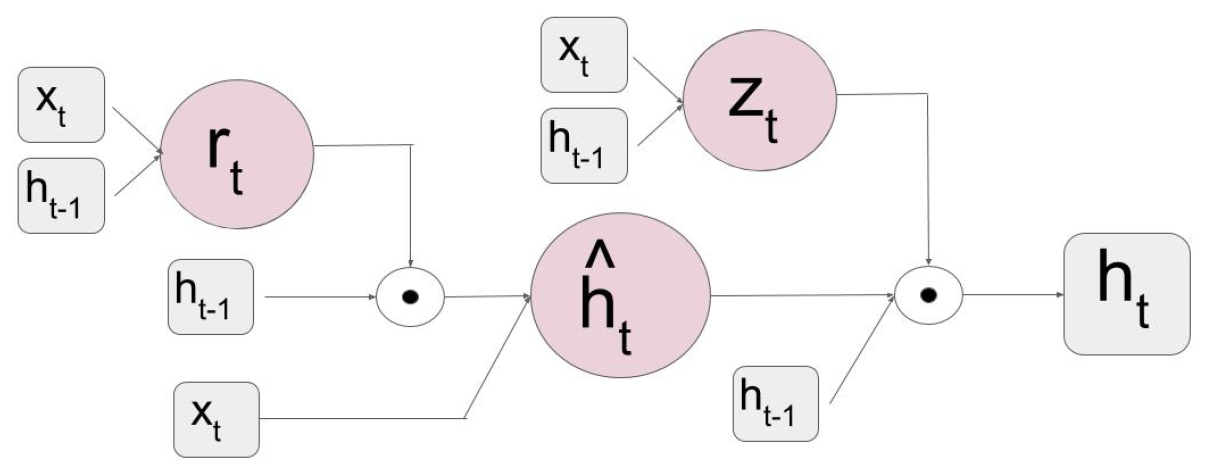
\includegraphics[scale=0.2]{gru.png} 
  \caption{GRU Architecture. \cite{rFCN}}
  \label{fig:gru}
\end{figure}

\subsection{Generative Adversarial Networks (GAN)}
\label{generative_adversarial_networks}
Generative Adversarial Networks (GAN) \cite{gan2014} are composed of two models that are alternatively trained to compete with each other. The generator $G$ is optimized to reproduce the true data distribution pdata by generating images that are difficult for the discriminator $D$ to differentiate from real images. Meanwhile, $D$ is optimized to distinguish real images and synthetic images generated by $G$. Overall, the training procedure is similar to a two-player min-max game with the following objective function,
$$\mathop{min}_{G} \mathop{min}_{D} V(D,G) = \mathbb{E}_{x~p_{data}} [log D(x)] + \mathbb{E}_{z~p_z} [log (1-G(z))]$$
where $x$ is a real image from the true data distribution $p_{data}$, and $z$ is a noise vector sampled from distribution $p_z$ (e.g., uniform or Gaussian distribution). 
\\\\
Conditional GAN \cite{faceGan2015, condGan2014} is an extension of GAN where both the generator and discriminator receive additional conditioning variables $c$, yielding $G(z,c)$ and $D(x,c)$. This formulation allows $G$ to generate images conditioned on variables $c$.


%%%%%%%%%%%%%%%%%%%%%%%%%%%%%%%%%%%%
%
%				Section: Our Approach
%
%%%%%%%%%%%%%%%%%%%%%%%%%%%%%%%%%%%%
\section{Our Approach}
\label{our_approach}
In our problem, we are given a pre-condition either in the form of an action class name, fMRI signal or textual description and we need to generate a sequence of video frames which will be coherent with the given pre-condition. First, we will discuss how we can generate a high resolution frame independently based on the pre-condition using a stacked adversarial network. Then we will discuss how we can make a recurrent fully convolutional network so we can propagate the context to generate the next frame. Finally, we will describe our recurrent stacked adversarial network to generate videos based on pre-conditions.

\subsection{Stacked Adversarial Network}
To generate a video first, we need to learn to generate a single frame from the pre-condition. We have adapted the  StackGAN adversarial network model \cite{stackGAN} for this problem, as it can generate photo-realistic images from sentence descriptions. At first stage, this model generates an image based on the encoded text and a random vector. Then the generated image in the first stage is used as the input with the encoded text vector to the second stage adversarial network to generate a photo-realistic image. The architecture of the model can be seen in Figure \ref{stackgan}.

\begin{figure}[h]
  \centering
  %%\fbox{\rule[-.5cm]{0cm}{4cm} \rule[-.5cm]{4cm}{0cm}}
  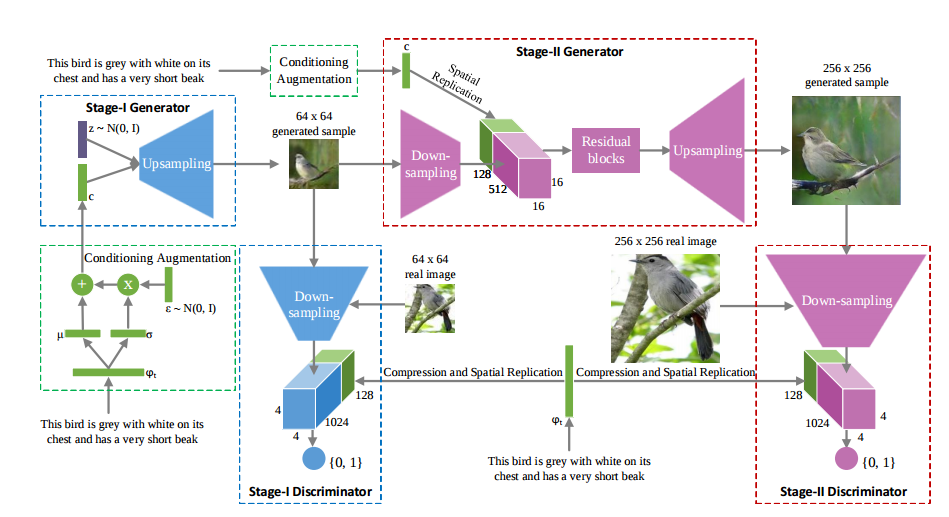
\includegraphics[scale=0.4]{stackgan.png} 
  \caption{The architecture of the StackGAN from \cite{stackGAN}. The Stage-I generator draws a low resolution image by sketching rough shape and basic colors of the object from the given text and painting the background from a random noise vector. The Stage-II generator generates a high resolution image with photo-realistic details by conditioning on both the Stage-I result and the text again.}
    \label{stackgan}
\end{figure}

\subsubsection{Stage-I GAN}
As shown in Figure \ref{stackgan}, the conditioning text description $t$ is first encoded by an encoder, yielding a text embedding $\varphi_t$. In previous works \cite{bayes2014, learn2016}, the text embedding is nonlinearly transformed to generate conditioning latent variables for the generator. However, latent space conditioned on text is usually high dimensional (> 100 dimensions). With limited amount of data, it usually causes discontinuity in the latent data manifold, which is not desirable for learning the generator.
\\
To mitigate this problem, we introduce a conditioning augmentation technique to produce more conditioning variables for the generator. We randomly sample latent variables from an independent Gaussian distribution $N(\mu(\varphi_t), \Sigma(\varphi_t))$, where the mean $\mu(\varphi_t)$ and diagonal covariance matrix $ \Sigma(\varphi_t)$ are functions of the text embedding $\varphi_t$. The proposed formulation encourages robustness to small perturbations along the conditioning manifold, and thus yields more training pairs given a small number of image-text pairs. To further enforce the smoothness over the conditioning manifold and avoid overfitting \cite{tutorial2016,autoEncod2016}, we add the following regularization term to the objective of the generator during training,
$$D_{KL}( N(\mu(\varphi_t), \Sigma(\varphi_t)) || N(0,I))$$
which is the Kullback-Leibler divergence (KL divergence) between the standard Gaussian distribution and the conditioning Gaussian distribution.
\\\\
Conditioned on Gaussian latent variables $c_0$, {Stage-I RSGAN} trains discriminator $D_0$ and generator $G_0$ by alternatively maximizing $\mathcal{L_\mathnormal{D_0}}$ and minimizing $\mathcal{L_\mathnormal{G_0}}$.

$$\mathcal{L_\mathnormal{D_0}} = \mathbb{E_\mathnormal{(I_0,t) \sim p_{data} }} [log D_0(I_0,\varphi_t)] + \mathbb{E_\mathnormal{z \sim p_z, t \sim p_{data} }} [log (1-D_0(G_0(z,c_0), \varphi_t))]$$
$$\mathcal{L_\mathnormal{G_0}} =  \mathbb{E_\mathnormal{z \sim p_z, t \sim p_{data} }} [log (1-D_0(G_0(z,c_0), \varphi_t))] + \lambda D_{KL} (\mathcal{N}(\mu_0(\varphi_t), \Sigma_0 (\varphi_t)) || \mathcal{N}(0,I))$$

where the real image $I_0$ and the text description $t$ are from the true data distribution $p_{data}$ $z$ is a noise vector randomly sampled from a given distribution $p_z$ (e.g., Gaussian distribution used in this paper). $\lambda$ is a regularization parameter that controls the balance between the two terms of $\mathcal{L_\mathnormal{G_0}}$. We use $\lambda= 1$ for all our experiments. $\varphi_t$ is the text embedding, which is generated by a pre-trained encoder \cite{fineGrain2016} in this paper. Gaussian conditioning variables $c_0$ are sampled from $N(\mu_0(\varphi_t), \Sigma_0(\varphi_t))$ to reflect the text description. Using the reparameterization trick introduced in \cite{autoEncod2014}, both $\mu_0(\varphi_t)$  and $\Sigma_0(\varphi_t)$ are learned jointly with the rest of the network.

\paragraph{Model Architecture}
For the generator, the text embedding $\varphi_t$ is fed into a fully connected layer to generate $\mu_0$ and $\sigma_0$ ($\sigma_0$are the values in the diagonal of $\Sigma_0$) for Gaussian distribution $N(\mu(\varphi_t), \Sigma(\varphi_t))$. 
Our $N_g$ dimensional conditioning vector $c_0$ is computed by $c0= \mu_0 + \sigma_0 \odot \epsilon$ (where $\odot$ is the element-wise multiplication, $\epsilon ~ N(0,I)$). Then, $c_0$ is concatenated with a $N_z$ dimensional noise vector to generate a $W_0 \times H_0$ image by a series of up-sampling blocks.
\\
For the discriminator, the text embedding $\varphi_t$ is first compressed to $N_d$ dimensions using a fully-connected layer and then spatially replicated to form a $M_d \times M_d \times N_d$ tensor. Meanwhile, the image is fed through a series of downsampling blocks until it has $M_d \times M_d$ spatial dimension.Then, the image filter map is concatenated along the channel dimension with the text tensor. The resulting tensor is further fed to a $1\times 1$ convolutional layer to jointly learn features across the image and the text. Finally, a fully connected layer with one node is used to produce the decision score.

\subsubsection{Stage-II GAN}
Low resolution images generated by Stage-I GAN lack vivid object parts and might also contain shape distortions. In addition, some details in the text might be omitted in the first stage. This is important information needed to generate a photo-realistic image. Stage-II GAN is built upon Stage-I GAN to generate photo-realistic high resolution images. It conditions on low resolution images generated by the previous stage, and also the text embedding again to correct defects in Stage-I results and encourage the model to extract previously ignored information in the text to generate more photo-realistic details.
\\\\
Conditioned on the low resulation sample $s_0$ and Gaussian latent variables $c$, discriminator $D$ and generator $G$ in {Stage-II RSGAN} is trained  by alternatively maximizing $\mathcal{L_\mathnormal{D}}$ and minimizing $\mathcal{L_\mathnormal{G}}$.

$$\mathcal{L_\mathnormal{D}} = \mathbb{E_\mathnormal{(I,t) \sim p_{data} }} [log D(I,\varphi_t)] + \mathbb{E_\mathnormal{s_0 \sim pG_0, t \sim p_{data} }} [log (1-D(G(s_0,c), \varphi_t))]$$
$$\mathcal{L_\mathnormal{G}} =  \mathbb{E_\mathnormal{s_0 \sim pG_0, t \sim p_{data} }} [log (1-D(G(s_0,c), \varphi_t))] + \lambda D_{KL} (\mathcal{N}(\mu(\varphi_t), \Sigma (\varphi_t)) || \mathcal{N}(0,I))$$

where $s0 = G0(z,c_0)$ is generated by Stage-I GAN. Different from the original GAN formulation, the random noise $z$ is not used in this stage with the assumption that the randomness has already been preserved in $s_0$. Gaussian conditioning variables $c$ used in this stage and c0 used in Stage-I GAN share the same pre-trained text encoder, generating the same text embedding $\varphi_t$. But, they utilize different fully connected layers for generating different means and standard deviations. In this way, Stage-II GAN learns to capture useful information in the text embedding that is omitted by Stage-I GAN.

\paragraph{Model Architecture}
For the generator, similar to the previous stage, $\varphi_t$ is used to generate our $N_g$ dimensional
Gaussian conditioning vector $c$, which is spatially replicated to form a $M_g \times M_g \times N_g$ tensor. Meanwhile, the sample $s_0$ generated by Stage-I GAN is fed into several downsampling blocks until it has a spatial size of  $M_g \times M_g$. Then, the image filter map and the text tensor are concatenated along the channel dimension. The resulting tensor is fed into several residual blocks \cite{ percep2016, deepRes2016} to jointly encode the image and text features, and finally a series of up-sampling blocks are used to generate a $W\times H$ image.
\\
For the discriminator, its structure is similar to that of Stage-I discriminator with only extra down-sampling blocks since the image size is larger in this stage. To explicitly enforce GAN to learn better alignment between the image and the conditioning text, rather than using the naive discriminator, we adopt the matching-aware discriminator proposed by Reed et al. \cite{autoEncod2014} for both stages. During training, the discriminator takes real images and their corresponding text descriptions as positive sample pairs, whereas negative sample pairs consist of two groups. The first is real images with mismatched text embeddings, while the second is synthetic images with conditioning text embeddings.

\subsection{Recurrent Fully Convolutional Network}
Now to generate a video, we need to pass the contextual information from previous frames to the current frame so the frames are coherent to each other. For the discriminator network, we can do that using a regular LSTM network. The discriminator network generates a vector from the input images which can be transfered to the next instance of the discriminator. But the generator network is mostly a fully convolutional neural network, it is not straightforward to create a recursive model for the generator. We have considered the recurrent fully convolutional network \cite{rFCN} to solve this problem. The model uses convolutional gated recurrent units which establishes recurrent connections between the colvolutional layers. This model preserves the spatial information while passing context to the next LSTM unit and reduces the number oflearned parameters as well. The model is described in Figure \ref{recurrent_fcn}.

\begin{figure}[h]
  \centering
  %%\fbox{\rule[-.5cm]{0cm}{4cm} \rule[-.5cm]{4cm}{0cm}}
  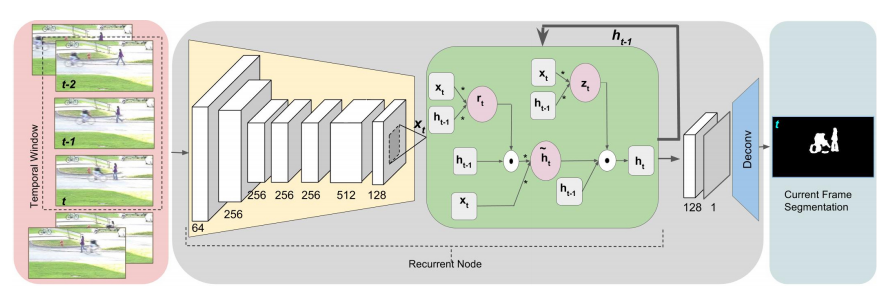
\includegraphics[scale=0.4]{recurrent_fcn.png} 
  \caption{The architecture of RFC-VGG from \cite{rFCN}. Images are fed frame by frame into a recurrent FCN. A Conv-GRU layer is applied on the feature maps produced by the preceding network at each frame.
The output of this layer goes to one more convolutional layer to generate heat maps. Finally, a
deconvolution layer up-samples the heat map to the desired spatial size.}
  \label{recurrent_fcn}
\end{figure}

\subsubsection{Convolutional Gated Recurrent Unit (Conv-GRU)}
Conventional recurrent units are capable of processing temporal data however, their architecture is not suitable for working on images/feature maps for two reasons. 1) weights matrix size, 2) ignoring spatial connectivity. Assume a case where a recurrent unit is placed after a feature map with the spatial size of $h\times w$ and have a number of channels $c$. After flattening, it will turn into a $c\times h.w$ long matrix. Therefore, weights of the recurrent unit will be of size $c\times (h.w)^2$ which is power four of spatial dimension. These matrices for weights can only be maintained for small feature maps. Even if the computation was not an issue, such design introduces too much variance in the network which prevents generalization. In Convolutional recurrent units, similar to regular convolutional layer,weights are three dimensional and they convolve with the input instead of dot product. Accordingly, the cell’s model, in the case of a GRU architecture, will turn into equations bellow where the dot products are replaced with convolutions. In this design, weights matrices are of size $k_h \times k_w \times c \times f$ where $k_h$, $k_w$, $c$ and $f$ are kernel’s height, kernel’s width, number of input channels, and number of filters, respectively. In Figure \ref{fig:gru} the operations applied on the input and the previous step will all be convolutions instead. Since we can assume spatial connectivity in feature maps, kernel size can be very small compared to feature map’s spatial size. Therefore, this architecture is much more efficient and weights are easier to learn due to smaller search space.
$$z_t = \sigma(W_{hz} * h_{t-1} + W_{xz} * x_t+ +b_z)$$
$$r_t = \sigma(W_{hr} * h_{t-1} + W_{xr} * x_t+ +b_r)$$
$$\hat{h_t} = \Phi (W_{h} * ( r_t \odot h_{t-1}) + W_x * x_t+ +b)$$
$$h_t = (1-z_t)\odot h_{t-1} + z \odot \hat{h_t}$$
We employ this approach for segmentation in a fully convolutional network. It is possible to apply this layer on either heat maps or feature maps. In the first case, the output of this layer will directly feed into the deconvolution layer and produces the pixel-wise probability map. In the latter case, at least one CNN layer needs to be used after the recurrent layer to convert its output feature maps to a heat map.

\subsection{Recurrent Stacked Generative Adversarial Network (RSGAN)}
Now, we have the models to generate individual images from the pre-condition and also we can connect this individual adversarial networks using recurrent connection. We combine these two models and propose the Recurrent Stacked Generative network (RSGAN) for conditional video generation. The model expands both in the temporal and spatial dimension. Each module in the first stage takes the encoded pre-condition and a random vector as input and passes a contextual matrix to the next module to generate a low resolution frame sequence. Then the modules in the second stage takes the encoded pre-condition and the low resolution output from the previous stage to generate a high resolution video sequence. The model is described in Figure \ref{RSGAN}.

\begin{figure}[h]
  \centering
  %%\fbox{\rule[-.5cm]{0cm}{4cm} \rule[-.5cm]{4cm}{0cm}}
  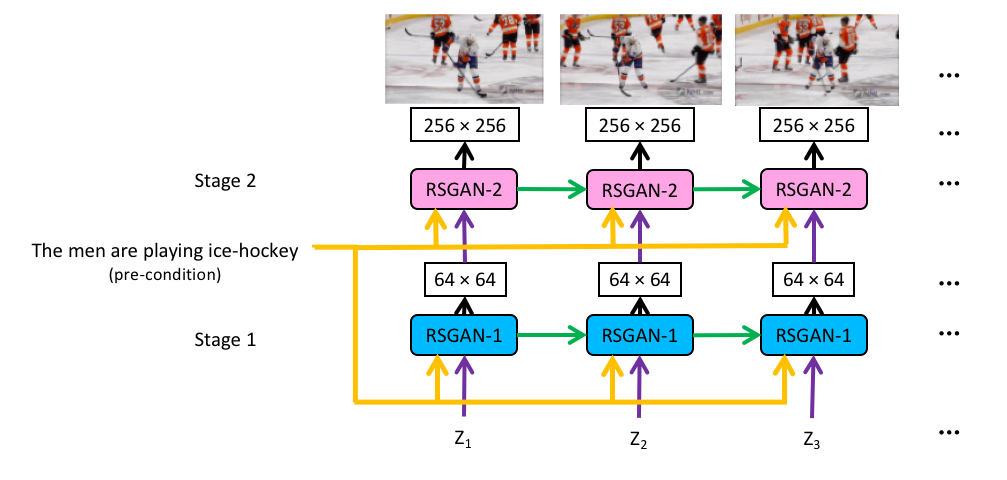
\includegraphics[scale=0.7]{rsgan_only.png} 
  \caption{The proposed Recurrent Stacked Generative network (RSGAN). The recurrent adversarial network modules at the first stage (RGAN-1) take the encoded pre-condition and a random vector $z_t$ and then produces a low resolution ($64 \times 64$) size image. The modules at stage-2 (RGAN-2) takes the generated image at stage-1 and the encoded pre-condition to generate a high resolution image ($256 \times 256$).}
    \label{RSGAN}
\end{figure}


%\subsubsection{Training} The model is trained using back propagation through time (bptt) and the usual adversarial training to train the recurrent generators and discriminators. 


%%%%%%%%%%%%%%%%%%%%%%%%%%%%%%%%%%%%
%
%				Section: Experiments
%
%%%%%%%%%%%%%%%%%%%%%%%%%%%%%%%%%%%%
\section{Experiments}
\label{experiments}
This section presents our experiments and results. First, we describe the datasets that we used then, we discuss our training methods and implemented hyper-parameters settings. Finally, quantitative and qualitative results are shown.

\subsection{Datasets}
In this paper four datasets are used: 1) NTU RGB+D Action Recognition Dataset, 2) UCF-101 Dataset.

\subsubsection{NTU RGB+D Action Recognition Dataset}
NTU RGB+D action recognition dataset consists of 56,880 action samples containing RGB videos, depth map sequences, 3D skeletal data, and infrared videos for each sample \cite{NTU}. This dataset is captured by 3 Microsoft Kinect v.2 cameras concurrently. The resolution of RGB videos are $1920 \times 1080$, depth maps and IR videos are all in $512 \times 424$, and 3D skeletal data contains the three dimensional locations of 25 major body joints, at each frame.

\subsubsection{UCF-101 Dataset}
%The UCF-101 \cite{uCF101} dataset contains short videos of 101 action classes. 
UCF101 \cite{uCF101} dataset is an action recognition data set of realistic action videos, collected from YouTube, having 101 action categories. With 13320 videos from 101 action categories, UCF101 gives the largest diversity in terms of actions and with the presence of large variations in camera motion, object appearance and pose, object scale, viewpoint, cluttered background, illumination conditions, etc. The videos in 101 action categories are grouped into 25 groups, where each group can consist of 4-7 videos of an action. The videos from the same group may share some common features, such as similar background, similar viewpoint, etc. The action categories can be divided into five types: 1)Human-Object Interaction 2) Body-Motion Only 3) Human-Human Interaction 4) Playing Musical Instruments 5) Sports. 

%\subsection{VIM-2 Dataset}
%VIM-2 dataset \cite{recVEBA} contains 7200 seconds of training and 540 seconds of test fMRI BOLD (blood oxygen level) signals and corresponding 15 frames of stimulation for each second. We will use the fMRI signals from the early visual area (V1, V2, V3, V3a, V3b) as our pre-condition to reproduce the video stimulations.

%\subsubsection{Large Scale Movie Description Dataset}
%Finally, we will use the Large Scale Movie Description Dataset \cite{movieDes} which contains 4-5 seconds videos from movies and their textual descriptions. We will use the Skip-Thought vector to encode the sentence descriptions and use them as pre-conditions.

\subsection{Evaluation Metrics}
To our knowledge, there is no existing published paper or method that accommodates RSGAN architecture and its performace.  open source framework that accommodates RFCNN architecture. So  as the baseline, we utilize only Stage-I GAN of our Stack-GAN for generating $64 \times 64$ images to investigate whether the stack structure is beneficial. Then we modify our Stack-GAN to generate $128 \times 128$ images to investigate whether larger images by our method results in clearer images. And we input text at both stages for generating images of better quality.
\\\\
It is difficult to evaluate the performance of generative models (e.g., GAN). Asking human annotators to determine the visual quality of samples is most intuitive and reliable. We also choose a recently proposed numerical assessment approach \textit{inception score} \cite{improvGan2016} for quantitative evaluation,
$$ I = exp \Big(\mathbb{E}_x D_{KL} \big(p(y|\textbf{x}) || p(y)) \big) \Big)$$
\\
where $x$ denotes one generated sample, and $y$ is the label predicted by the Inception model [28]. The intuition behind this metric is that good models should generate diverse but meaningful images. Therefore, the KL divergence between the marginal distribution $p(y)$ and the conditional distribution $p(y|\textbf{x})$ should be large.

\subsection{Training Methods and Implementation}
From NTU RGB+D Dataset, we use only the 3D skeletal videos which are 2-5s long each and each video is labeled by an action label. Skeletal video frames are based on the locations of the detected body joints, and join them by a line. For good performance, we use mask to remove the background and less important parts of the depth maps and to improve the compression rate.

\paragraph{StanGan Implementaion}
The up-sampling blocks consist of the nearest-neighbor upsampling followed by a $3 \times 3$ stride 1 convolution. Batch normalization \cite{batchNorm2014} and ReLU activation are applied after every convolution except the last one. The residual blocks consist of $3 \times 3$ stride 1 convolutions, Batch normalization and ReLU. Two residual blocks are used in $128 \times 128$ StackGAN models while four are used in $256 \times 256$ models. The down-sampling blocks consist of $4 \times 4$ stride 2 convolutions, Batch normalization and LeakyReLU \cite{rectifier2013, rectifierConv2015}, except that the first one does not have Batch normalization.
\\
By default, $N_g = 128, N_z = 100, M_g = 16, M_d = 4, N_d = 128, W_0 = H_0 = 64 and W = H = 256$. For training, we first iteratively train $D_0$ and $G_0$ of Stage-I GAN for 600 epochs by fixing Stage-II GAN. Then we iteratively train D and G of Stage-II GAN for another 600 epochs by fixing Stage-I GAN. All networks are trained using ADAM solver with batch size 64 and an initial learning rate of 0.0002. The learning rate is decayed to $\frac{1}{2}$ of its previous value every 100 epochs.

\paragraph{Conv-GRU Implementaion}
RFC-VGG in figure \ref{conv-gru} is based on VGG-F \cite{imgRecog2014} network. Initializing weights of our filters by VGG-F trained weights, alleviates over-fitting problems as these weights are the result of extensive training on the imagenet. The network is cast to a fully convolutional one by replacing the fully connected layers with convolutional layers. The last two pooling layers are dropped from VGG-F to allow a finer frame. Then a convolutional gated recurrent unit is used followed by one convolutional layer and then deconvolution for up-sampling. Figure \ref{recurrent_fcn} shows the detailed architecture of RFC-VGG.
\begin{figure}[h]
  \centering
  %%\fbox{\rule[-.5cm]{0cm}{4cm} \rule[-.5cm]{4cm}{0cm}}
  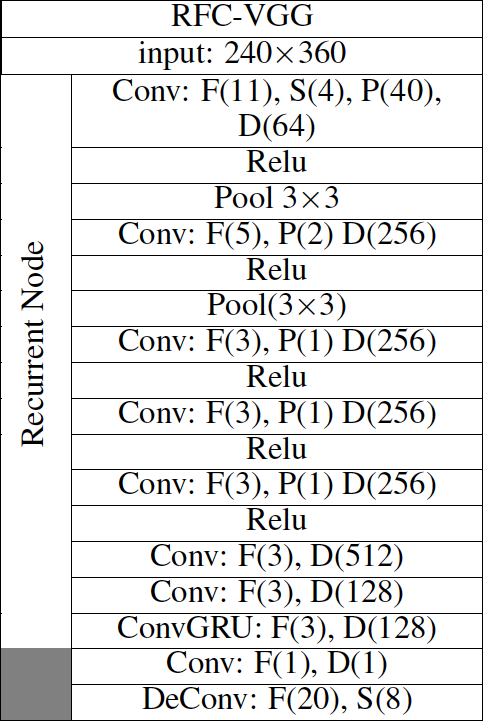
\includegraphics[scale=0.2]{conv-gru.png} 
  \caption{Proposed Conv-GRU networks. $F(n)$ denotes filter size of $n \times n$. $P(n)$ denotes total of $n$ zero padding around the feature map. $S(n)$ denotes stride of length $n$ for the convolution. $D(n)$ denotes number of output feature maps from a particular layer $n$ for a layer (number of feature maps is same as previous layer if $D$ is not mentioned).}
    \label{conv-gru}
\end{figure}

\subsection{Qualitative Results}

\paragraph{NTU RGB+D Action Recognition Dataset}
The main experiments are conducted using Adadelta \cite{adaDelta2012} for optimization that practically gave much faster convergence than standard stochastic gradient descent. The logistic loss function is used and the maximum number of epochs used for the training is 500.

\begin{figure}[htbp]
    \centering
	\subfloat[ Action: Drink water.\label{fig:1a}]{\includegraphics[width=0.5\textwidth]{"drink water"}}\hfill
	\subfloat[Action: Drop.\label{fig:1b}] {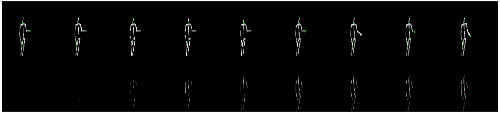
\includegraphics[width=0.5\textwidth]{drop}}\hfill
	\subfloat[Action: Point finger at the other person.\label{fig:1c}]{\includegraphics[width=0.5\textwidth]{"point finger at the other person"}}
	\subfloat[Action: Reading.\label{fig:1b}] {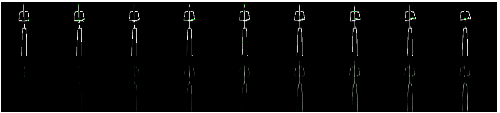
\includegraphics[width=0.5\textwidth]{reading}}\hfill
	\subfloat[Action: Slapping other person.\label{fig:1b}] {\includegraphics[width=0.5\textwidth]{"slapping other person"}}\hfill
	\subfloat[Action: Tablet.\label{fig:1b}] {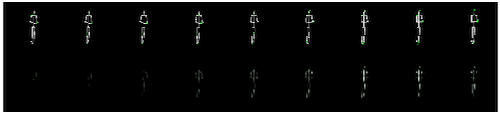
\includegraphics[width=0.5\textwidth]{tablet}}\hfill
	\subfloat[Action: Writing.\label{fig:1b}] {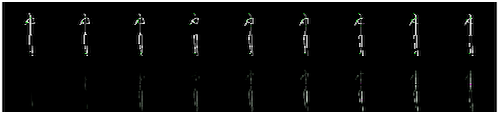
\includegraphics[width=0.5\textwidth]{writing}}\hfill
	
	\caption{Example results by our proposed RSGAN. The first row is the ground truth, and the second row is the output frame of RSGAN.} \label{fig:1}    

\end{figure}

\paragraph{UCF-101 Dataset}
UCF-101 videos are more realistic and, has complex texture and sturctural relations among various objects. We train our RSGAN using first 90 action classes and later try to generate videos for other 11 classes. We input the word-vector representation of the action class names and use those as the pre-conditions to generate the videos. 

\begin{figure}[htbp]
    \centering
	\subfloat[ \label{fig:1aUCF101}]{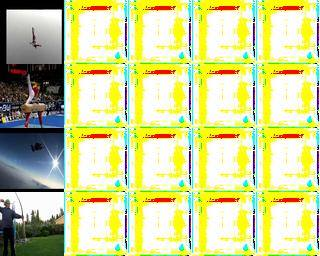
\includegraphics[width=0.49\textwidth]{UCF101-dance}}\hfill
	\subfloat[ \label{fig:1bUCF101}] {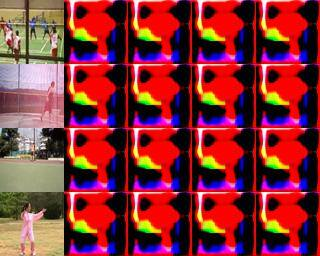
\includegraphics[width=0.49\textwidth]{UCF101-stand}}\hfill
	
	\caption{Example results by our proposed RSGAN. The first coulmn is a ground truth frame of the input action class, and the other columns are the output frames of RSGAN.} \label{fig:1}    

\end{figure}
\FloatBarrier


%%%%%%%%%%%%%%%%%%%%%%%%%%%%%%%%%%%%
%
%				Section: Conclusion
%
%%%%%%%%%%%%%%%%%%%%%%%%%%%%%%%%%%%%
\section{Conclusion and Future Works}
\label{conclusion}
We have proposed a novel adversarial network based model to generate videos based on a given condition. Our model can generate video frames which are coherent and consistent to the given condition. Since no published work is still avaiable to address this pre-condition video, it is very difficult to compare performance with. Right now, for simple detailed video like, NTU RGB+D Action Recognition Dataset, RSGAN is most likely generate somewhat consistant video frames. But for complex scene of UCF-101 Dataset, the result is very poor. In future, we are like to investigate whether applying batch normalization in GRU can imporve the result like it does in StanGan module. And if we get any success in that, then we will extend our pre-condition to VIM-2 dataset \cite{recVEBA}. In this dataset, fMRI BOLD signals from human brain will be used to simulate video frames.

%\section*{References}
\small
\bibliographystyle{abbrv}
\bibliography{project_report}

\end{document}